\section{Introduction}\label{sec:intro}

Feature-universality studies pair sparse-autoencoder (SAE) features of separately trained
networks by their highest activation correlation
\citep{bricken2023monosemanticity,wang2025universality,lan2024universal}, and read close pairs as evidence of shared features.
On C4, the released SAEs of Gemma-2-9B and Mistral-7B, two families with different tokenizers,
each have an obituary feature, and the two features' five most-activating documents are the same five (\Cref{app:matched-examples}). Such pairs are cheap to manufacture: two sets of $1{,}500$ features
reciprocally match about half of each other under idealized chance (\Cref{prop:null}), and any
document property both models encode (length, topic, vocabulary, the current word) can make
features coactivate with no shared feature behind them.

\begin{figure}[t]
\centering
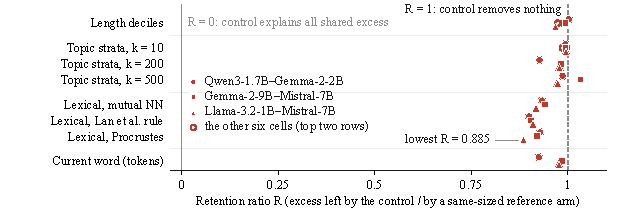
\includegraphics[width=\textwidth]{figures/fig1_20261010/fig1.pdf}
\caption{\textbf{Every control we ran leaves nearly all of the cross-model shared excess: retention ratios sit near $R=1$, far from $R=0$.} $R$ \eqref{eq:ratio} is the excess left after a control over that left by a same-sized reference arm; $R=1$ means the control removes nothing beyond its reference arm, and $R=0$ that the covariate, as the control captures it, explains all of the sharing. Top two rows: all nine cross-family cells (\Cref{tab:ninecell}); other rows: three representative cells (\Cref{tab:ladder}). Drawn by \texttt{code/figures/fig1\_control\_ladder\_20261010.py} from the \texttt{ninecell\_20260926/A\_*}, \texttt{lextok20k\_*}, \texttt{lanpair\_*}, \texttt{proclex\_*} and \texttt{tokaclean20k\_*} receipts.}
\label{fig:arc}\label{fig:controls-main}
\end{figure}

Sparse autoencoders and transcoders \citep{cunningham2023sparse,bricken2023monosemanticity,
ameisen2025attribution,lindsey2025biology} make such comparisons easy to run, and cross-model
matches are read as evidence of representational convergence
\citep{huh2024platonic,lan2024universal}. The published cross-model protocol pairs features
greedily and judges significance against random pairings, on same-tokenizer pairs and without
controls for shared document properties \citep{lan2024universal}. A pairing rule fit to the data inflates any statistic
computed on the same data \citep{kriegeskorte2009circular}: re-implemented without their
filters on three of our pairs (all but GPT-2$\leftrightarrow$Mistral-7B, which shows no signal above random), a null that permutes documents before the pairing step sits far above that random
baseline, so part of the signal above random (up to $94\%$ on templated prompts, less on C4) comes
from the pairing itself (\Cref{app:lan}). With their filters added, that share shrinks on templates
but does not vanish, and on C4 too few permuted pairs survive the filters to estimate it
(\Cref{app:lan_filters}). That protocol lacks a null that re-runs the pairing
rule, pairs scored on documents the rule never saw, and controls that hold named mundane causes fixed.

We add all three, on open-weight models, and apply controls built to kill the signal
(\Cref{fig:arc}). It survives. In all nine cross-family cells across Gemma-2, Mistral, Qwen3
and Llama-3, pairs selected on half of a C4 slice still beat their null on the disjoint other
half (each at the floor of its permutation test; this follow-up was not pre-registered). On three representative
cells, fine topic strata, cross-fitted lexical residualization under three pairing rules, and
registered current-word conditioning at token level each leave a retention ratio of at least
$0.88$ against its reference arm. What survives is coactivation on shared inputs, not feature
identity: both cross-model ablation probes were inconclusive, and a dictionary confound (cells differ
in SAE dictionary, not only in model) blocks any capability-trend reading. The instruments
behind the positive can return a no: size- and sparsity-matched random directions fall below
their own null, Pythia-70M$\leftrightarrow$Mistral-7B falls to null on C4, and on
planted data the token-aligned analysis collapses a unigram-only signal while planted context
survives (\Cref{app:tokalign}).

\paragraph{Contributions.}
\begin{enumerate}[leftmargin=*,topsep=2pt,itemsep=1pt]
  \item \textbf{A reusable test that separates shared responses from named mundane correlates.} A
  re-matching permutation null, frozen pairs scored on disjoint documents, and controls read as retention
  ratios against a same-sized reference arm; two propositions show why, for any pairing rule, the null and
  frozen score carry no selection optimism while a re-selected score does (\Cref{sec:method}).
  \item \textbf{A scoped cross-model positive.} Coactivation on shared inputs in nine
  cross-family cells on held-out documents (non-pre-registered), three of them through the full control ladder (\Cref{fig:arc,fig:heldout-main},
  \Cref{tab:ladder}); not feature identity, composition, a capability trend, or shared computation.
  \item \textbf{Three rejections, each with the practice it implies.} The controls reject a
  Pythia-70M$\leftrightarrow$Mistral-7B match null on natural text (so recheck template matches on
  natural text), a depth-driven cross-lingual metric (so add a mismatched-concept control), and its
  depth-corrected residual at $206$ concept pairs and $17$ models (so use several English-only
  baselines) (\Cref{sec:results:secondary,sec:results:sae-matching}).
\end{enumerate}
